\documentclass[usenames, aspectratio=169]{beamer}

\usepackage{amsmath}
\usepackage{braket}
\usepackage{amsfonts}
\usepackage{tikz}
\usepackage{tkz-graph}
\usepackage{tikzpeople}
\usepackage{adjustbox}
\usepackage{subcaption}
\usepackage{svg}
\usepackage{graphicx}
\usepackage{media9}
\usepackage{float}
\usetikzlibrary{calc}
\usepackage{array}
\usepackage{efbox,graphicx}
\usepackage[normalem]{ulem}
\usepackage{verbatim}
\usepackage{ragged2e}
\usepackage{array}
\efboxsetup{linecolor=Green,linewidth=1.5pt, margin=0pt}

\usetikzlibrary{decorations.pathreplacing}

\newcommand\MemoryLayout[1]{
  \begin{tikzpicture}[scale=0.15]
    \draw[thick](0,0)--++(0,3)node[above]{$0$};
    \foreach \pt/\col/\lab [remember=\pt as \tp (initially 0)] in {#1} {
      \foreach \a [parse=true] in {\tp,...,\pt-1} {
        \draw[fill=\col](-\a, 0) rectangle ++(-1,2);
      }
      \draw[thick](-\pt,0)--++(0,3)node[above]{$\pt$};
      \if\lab\relax\relax\else
        \draw[thick,decorate, decoration={amplitude=1mm}]
        (-\tp,-0.2)--node[below=1mm]{\lab} (-\pt,-0.2);
      \fi
    }
  \end{tikzpicture}
}


\newcommand{\pslsq}[4]{
\begin{frame}
    \frametitle{#1} 
    \includegraphics[width=.7\linewidth]{#3}
    #4  
  \end{frame}
}

\newcommand{\psls}[4]{
  \begin{frame}
    \frametitle{#1} 
    \begin{columns}[t]
      \begin{column}{.48\textwidth}
        #4
      \end{column}
      \begin{column}{.52\textwidth}
        \adjincludegraphics[width=.98\linewidth, valign=t]{#3}
      \end{column} 
    \end{columns}
  \end{frame}
}
\usepackage{sagetex}
%\usepackage{libertine}
%\usepackage{emerald}
%\usepackage[T1]{fontenc}
\usetheme[progressbar=frametitle]{metropolis}
\setbeamercolor{block title}{use=structure,fg=white,bg=structure.fg!75!black}
\setbeamercolor{block body}{parent=normal text,use=block title,bg=block title.bg!10!bg}

%\usetheme{EastLansing}
\title[Understanding Quantumness And Testability.] % (optional, only for long titles)
{Understanding Quantumness And Testability.}

\subtitle{  }
\author[D.~Ponarovsky] % (optional, for multiple authors)
	{D.~Ponarovsky\inst{1}}

\institute[HUJI] % (optional)
{  Faculty of Computer Science\newline
  Hebrew University of Jerusalem
}
\date[2023] % (optional)
{Master-Exam-Huji.}
\subject{Understanding Quantumness And Testability.}

\begin{document}
\input{sageutil.py}

\tikzset{
    LabelStyle/.append style = {  minimum width = 2em, fill = white},
    VertexStyle/.append style = { inner sep=5pt,
        font = \Large\bfseries},
    EdgeStyle/.append style = {->} % added blue
}

\begin{frame}
  \maketitle
\end{frame}
%\pslsq{Today.}{0.3}{controller.png}{}
%\pslsq{Today.}{0.5}{controller-2-out.png}{}

\begin{frame}
  \frametitle{ Today. }
  \begin{itemize}
    \item<1-> Brif Review of Coding. 
    \item<2-> Quantum Error Correction Codes.
    \item<3->Good Classical Locally Testabile Codes and Good Qauntum LDPC.
  \end{itemize} 
\end{frame}


\begin{frame}
  \frametitle{Introduction.}
  \includegraphics[width=.7\linewidth]{./Assumption-out.png}
\end{frame}



\begin{frame}
  \frametitle{ Coding. }
  \begin{center}
  
\begin{tikzpicture}
    \node[name=b, bob,monitor,minimum size=1cm,xshift=-7.2cm]{};
    \node[name= a, alice,monitor, mirrored,minimum size=1cm]{};
    \node (C) at (-3,0) {C};
    \draw[ -> ] (b.mouth) + (1,0) to (C)  ; 
  \end{tikzpicture}
\end{center}
\end{frame}

\begin{frame}
  \frametitle{ Coding. }
  Can we come up with a code that tolerates $*$ bits flip? 
\end{frame} 

\begin{frame}
  \frametitle{ Coding. }
\begin{definition} 
  Let $n \in \mathbb{N}$ and $\rho, \delta\in \left( 0,1 \right)$. We say that $C$ is a \textbf{binary linear code} with parameters $[n, \rho n, \delta n]$. If $C$ is a subspace of $\mathbb{F}_{2}^{n}$, and the dimension of $C$ is at least $\rho n$. In addition, we call the vectors belong to $C$ \textit{codewords} and define the distance of $C$ to be the minimal number of different bits between any codewords pair of $C$.   
  \end{definition}
\end{frame} 

\begin{frame}
  \frametitle{ Coding. }
\begin{definition} 
  A \textbf{family of codes} is an infinite series of codes. Additionally, suppose the rates and relative distances converge into constant values $\rho,\delta$. In that case, we abuse the notation and call that family of codes a code with $[n, \rho n, \delta n]$ for fixed $\rho, \delta\in [ 0,1 )$, and infinite integers $n \in \mathbb{N}$.     
  \end{definition}
\begin{definition} 
  We will say that a family of codes is a \textbf{good code} if its parameters converge into positive values. 
  \end{definition}
\end{frame} 

\begin{frame}
  \frametitle{ Coding. }
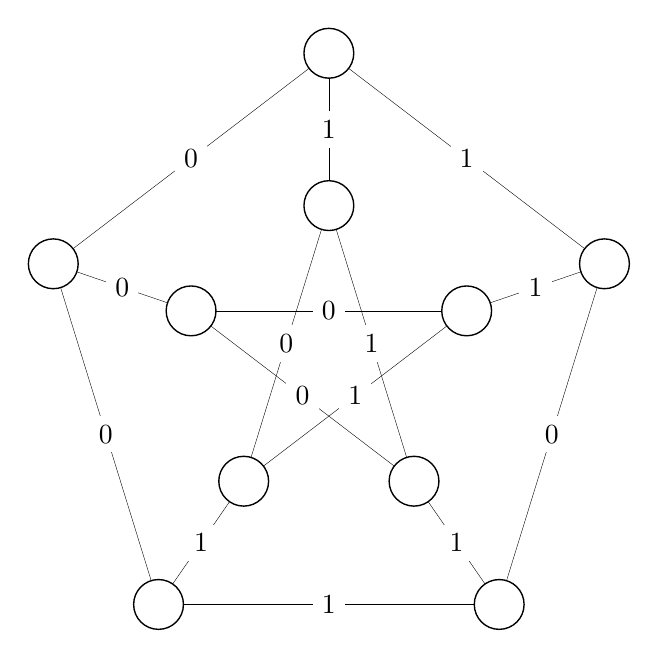
\begin{tikzpicture}
%\definecolor{cv0}{rgb}{0.0,0.0,0.0}
%\definecolor{cfv0}{rgb}{1.0,1.0,1.0}
%\definecolor{cv1}{rgb}{0.0,0.0,0.0}
%\definecolor{cfv1}{rgb}{1.0,1.0,1.0}
%\definecolor{cv2}{rgb}{0.0,0.0,0.0}
%\definecolor{cfv2}{rgb}{1.0,1.0,1.0}
%\definecolor{cv3}{rgb}{0.0,0.0,0.0}
%\definecolor{cfv3}{rgb}{1.0,1.0,1.0}
%\definecolor{cv4}{rgb}{0.0,0.0,0.0}
%\definecolor{cfv4}{rgb}{1.0,1.0,1.0}
%\definecolor{cv5}{rgb}{0.0,0.0,0.0}
%\definecolor{cfv5}{rgb}{1.0,1.0,1.0}
%\definecolor{cv6}{rgb}{0.0,0.0,0.0}
%\definecolor{cfv6}{rgb}{1.0,1.0,1.0}
%\definecolor{cv7}{rgb}{0.0,0.0,0.0}
%\definecolor{cfv7}{rgb}{1.0,1.0,1.0}
%\definecolor{cv8}{rgb}{0.0,0.0,0.0}
%\definecolor{cfv8}{rgb}{1.0,1.0,1.0}
%\definecolor{cv9}{rgb}{0.0,0.0,0.0}
%\definecolor{cfv9}{rgb}{1.0,1.0,1.0}
%\definecolor{cv0v1}{rgb}{0.0,0.0,0.0}
%\definecolor{clv0v1}{rgb}{0.0,0.0,0.0}
%\definecolor{cv0v4}{rgb}{0.0,0.0,0.0}
%\definecolor{clv0v4}{rgb}{0.0,0.0,0.0}
%\definecolor{cv0v5}{rgb}{0.0,0.0,0.0}
%\definecolor{clv0v5}{rgb}{0.0,0.0,0.0}
%\definecolor{cv1v2}{rgb}{0.0,0.0,0.0}
%\definecolor{clv1v2}{rgb}{0.0,0.0,0.0}
%\definecolor{cv1v6}{rgb}{0.0,0.0,0.0}
%\definecolor{clv1v6}{rgb}{0.0,0.0,0.0}
%\definecolor{cv2v3}{rgb}{0.0,0.0,0.0}
%\definecolor{clv2v3}{rgb}{0.0,0.0,0.0}
%\definecolor{cv2v7}{rgb}{0.0,0.0,0.0}
%\definecolor{clv2v7}{rgb}{0.0,0.0,0.0}
%\definecolor{cv3v4}{rgb}{0.0,0.0,0.0}
%\definecolor{clv3v4}{rgb}{0.0,0.0,0.0}
%\definecolor{cv3v8}{rgb}{0.0,0.0,0.0}
%\definecolor{clv3v8}{rgb}{0.0,0.0,0.0}
%\definecolor{cv4v9}{rgb}{0.0,0.0,0.0}
%\definecolor{clv4v9}{rgb}{0.0,0.0,0.0}
%\definecolor{cv5v7}{rgb}{0.0,0.0,0.0}
%\definecolor{clv5v7}{rgb}{0.0,0.0,0.0}
%\definecolor{cv5v8}{rgb}{0.0,0.0,0.0}
%\definecolor{clv5v8}{rgb}{0.0,0.0,0.0}
%\definecolor{cv6v8}{rgb}{0.0,0.0,0.0}
%\definecolor{clv6v8}{rgb}{0.0,0.0,0.0}
%\definecolor{cv6v9}{rgb}{0.0,0.0,0.0}
%\definecolor{clv6v9}{rgb}{0.0,0.0,0.0}
%\definecolor{cv7v9}{rgb}{0.0,0.0,0.0}
%\definecolor{clv7v9}{rgb}{0.0,0.0,0.0}
%
\Vertex[style={minimum size=0.01cm,shape=circle},NoLabel,x=3.5cm,y=7.0cm]{v0}
\Vertex[style={minimum size=0.01cm,shape=circle},NoLabel,x=0.0cm,y=4.3262cm]{v1}
\Vertex[style={minimum size=0.01cm,shape=circle},NoLabel,x=1.3369cm,y=0.0cm]{v2}
\Vertex[style={minimum size=0.01cm,shape=circle},NoLabel,x=5.6631cm,y=0.0cm]{v3}
\Vertex[style={minimum size=0.01cm,shape=circle},NoLabel,x=7.0cm,y=4.3262cm]{v4}
\Vertex[style={minimum size=0.01cm,shape=circle},NoLabel,x=3.5cm,y=5.0652cm]{v5}
\Vertex[style={minimum size=0.01cm,shape=circle},NoLabel,x=1.75cm,y=3.7284cm]{v6}
\Vertex[style={minimum size=0.01cm,shape=circle},NoLabel,x=2.4184cm,y=1.5652cm]{v7}
\Vertex[style={minimum size=0.01cm,shape=circle},NoLabel,x=4.5816cm,y=1.5652cm]{v8}
\Vertex[style={minimum size=0.01cm,shape=circle},NoLabel,x=5.25cm,y=3.7284cm]{v9}
%
\Edge[lw=0.005cm,labelstyle={pos=0.5},label=\hbox{$0$},](v0)(v1)
\Edge[lw=0.005cm,labelstyle={pos=0.5},label=\hbox{$1$},](v0)(v4)
\Edge[lw=0.005cm,labelstyle={pos=0.5},label=\hbox{$1$},](v0)(v5)
\Edge[lw=0.005cm,labelstyle={pos=0.5},label=\hbox{$0$},](v1)(v2)
\Edge[lw=0.005cm,labelstyle={pos=0.5},label=\hbox{$0$},](v1)(v6)
\Edge[lw=0.005cm,labelstyle={pos=0.5},label=\hbox{$1$},](v2)(v3)
\Edge[lw=0.005cm,labelstyle={pos=0.5},label=\hbox{$1$},](v2)(v7)
\Edge[lw=0.005cm,labelstyle={pos=0.5},label=\hbox{$0$},](v3)(v4)
\Edge[lw=0.005cm,labelstyle={pos=0.5},label=\hbox{$1$},](v3)(v8)
\Edge[lw=0.005cm,labelstyle={pos=0.5},label=\hbox{$1$},](v4)(v9)
\Edge[lw=0.005cm,labelstyle={pos=0.5},label=\hbox{$0$},](v5)(v7)
\Edge[lw=0.005cm,labelstyle={pos=0.5},label=\hbox{$1$},](v5)(v8)
\Edge[lw=0.005cm,labelstyle={pos=0.5},label=\hbox{$0$},](v6)(v8)
\Edge[lw=0.005cm,labelstyle={pos=0.5},label=\hbox{$0$},](v6)(v9)
\Edge[lw=0.005cm,labelstyle={pos=0.5},label=\hbox{$1$},](v7)(v9)
%
\end{tikzpicture}
\end{frame}


\begin{frame}
  \frametitle{ Quantum Error Correction Codes. }
\end{frame} 

\begin{frame}
  \frametitle{ Quantum Error Correction Codes. }

\begin{definition}[CSS Code]
  Let $C_{X}, C_{Z}$ classical linear codes such that $C_{Z}^{\perp} \subset C_{X}$ define the $Q\left( C_{X},C_{Z} \right)$ to be all the code words with following structure:
  \begin{equation*}
    \begin{split}
    \ket { \mathbf{ x } } := \ket { x + C_{Z}^{\perp} } = \frac{1}{\sqrt{C_{Z}^{\perp}}} \sum_{z \in C_{Z}^{\perp}}{ \ket{ x + z }} 
    \end{split}
  \end{equation*}
\end{definition}
\end{frame} 

\begin{frame}
  \frametitle{ Quantum Error Correction Codes. }
  \begin{center}
    \begin{figure}[H]
  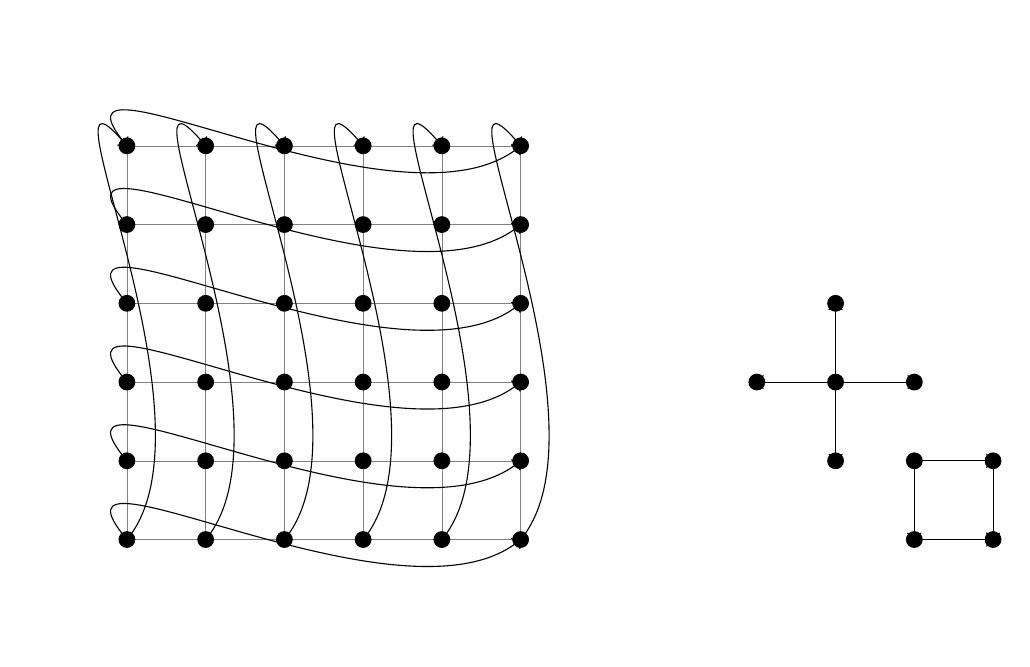
\begin{tikzpicture}
  \draw[step=1cm,gray,very thin] (0,0) grid (5,5);
  \foreach \x in {0,1,2,3,4,5}
  \foreach \y in {0,1,2,3,4,5}
  {
  \node[draw,circle,inner sep=2pt,fill] at (\x,\y) {};
}
\draw[ -> ]  (0,0) to [out=50, in=130] (0,5);
\draw[ -> ]  (1,0) to [out=50, in=130] (1,5);
\draw[ -> ]  (2,0) to [out=50, in=130] (2,5);
\draw[ -> ]  (3,0) to [out=50, in=130] (3,5);
\draw[ -> ]  (4,0) to [out=50, in=130] (4,5);
\draw[ -> ]  (5,0) to [out=50, in=130] (5,5);
\draw[ -> ]  (0,5) to [out=130, in=220] (5,5);
\draw[ -> ]  (0,4) to [out=130, in=220] (5,4);
\draw[ -> ]  (0,3) to [out=130, in=220] (5,3);
\draw[ -> ]  (0,2) to [out=130, in=220] (5,2);
\draw[ -> ]  (0,1) to [out=130, in=220] (5,1);
\draw[ -> ]  (0,0) to [out=130, in=220] (5,0);

\node[draw,circle,inner sep=2pt,fill] at (9,2) {};
\node[draw,circle,inner sep=2pt,fill] at (10,2) {};
\node[draw,circle,inner sep=2pt,fill] at (8,2) {};
\node[draw,circle,inner sep=2pt,fill] at (9,1) {};
\node[draw,circle,inner sep=2pt,fill] at (9,3) {};
\draw[ -> ]  (9,2) to (10,2);
\draw[ -> ]  (9,2) to (8,2);
\draw[ -> ]  (9,2) to (9,1);
\draw[ -> ]  (9,2) to (9,3);
%\draw[ -> ]  (9,2) to (5,0);

\node[draw,circle,inner sep=2pt,fill] at (10,1) {};
\node[draw,circle,inner sep=2pt,fill] at (11,1) {};
\node[draw,circle,inner sep=2pt,fill] at (10,0) {};
\node[draw,circle,inner sep=2pt,fill] at (11,0) {};
\draw[ -> ]  (10,1) to (11,1);
\draw[ -> ]  (10,1) to (10,0);
\draw[ -> ]  (10,0) to (11,0);
\draw[ -> ]  (11,1) to (11,0);
\end{tikzpicture}
\caption{On the left is the Toric Graph. On the right are cross and face checks.}
\label{fig:Toric}
\end{figure}
\end{center}

\end{frame} 

\begin{frame}
  \frametitle{ Coding. }
\end{frame} 


\psls{BUS.}{0.3}{./Peterson-out.png}{ 
  \begin{itemize}[<+->]
    \item  A BUS is a communication pathway that transfers data between different components of a computer.
    \item  Buses connect IO devices such as keyboards, monitors, and printers to the computer's central processing unit (CPU).
    \item  Buses provide a standardized way for different components to exchange data with each other, simplifying device connection and ensuring compatibility.
\end{itemize}
}



\end{document}
